\documentclass[1p]{elsarticle_modified}
%\bibliographystyle{elsarticle-num}

%\usepackage[colorlinks]{hyperref}
%\usepackage{abbrmath_seonhwa} %\Abb, \Ascr, \Acal ,\Abf, \Afrak
\usepackage{amsfonts}
\usepackage{amssymb}
\usepackage{amsmath}
\usepackage{amsthm}
\usepackage{scalefnt}
\usepackage{amsbsy}
\usepackage{kotex}
\usepackage{caption}
\usepackage{subfig}
\usepackage{color}
\usepackage{graphicx}
\usepackage{xcolor} %% white, black, red, green, blue, cyan, magenta, yellow
\usepackage{float}
\usepackage{setspace}
\usepackage{hyperref}

\usepackage{tikz}
\usetikzlibrary{arrows}

\usepackage{multirow}
\usepackage{array} % fixed length table
\usepackage{hhline}

%%%%%%%%%%%%%%%%%%%%%
\makeatletter
\renewcommand*\env@matrix[1][\arraystretch]{%
	\edef\arraystretch{#1}%
	\hskip -\arraycolsep
	\let\@ifnextchar\new@ifnextchar
	\array{*\c@MaxMatrixCols c}}
\makeatother %https://tex.stackexchange.com/questions/14071/how-can-i-increase-the-line-spacing-in-a-matrix
%%%%%%%%%%%%%%%

\usepackage[normalem]{ulem}

\newcommand{\msout}[1]{\ifmmode\text{\sout{\ensuremath{#1}}}\else\sout{#1}\fi}
%SOURCE: \msout is \stkout macro in https://tex.stackexchange.com/questions/20609/strikeout-in-math-mode

\newcommand{\cancel}[1]{
	\ifmmode
	{\color{red}\msout{#1}}
	\else
	{\color{red}\sout{#1}}
	\fi
}

\newcommand{\add}[1]{
	{\color{blue}\uwave{#1}}
}

\newcommand{\replace}[2]{
	\ifmmode
	{\color{red}\msout{#1}}{\color{blue}\uwave{#2}}
	\else
	{\color{red}\sout{#1}}{\color{blue}\uwave{#2}}
	\fi
}

\newcommand{\Sol}{\mathcal{S}} %segment
\newcommand{\D}{D} %diagram
\newcommand{\A}{\mathcal{A}} %arc


%%%%%%%%%%%%%%%%%%%%%%%%%%%%%5 test

\def\sl{\operatorname{\textup{SL}}(2,\Cbb)}
\def\psl{\operatorname{\textup{PSL}}(2,\Cbb)}
\def\quan{\mkern 1mu \triangleright \mkern 1mu}

\theoremstyle{definition}
\newtheorem{thm}{Theorem}[section]
\newtheorem{prop}[thm]{Proposition}
\newtheorem{lem}[thm]{Lemma}
\newtheorem{ques}[thm]{Question}
\newtheorem{cor}[thm]{Corollary}
\newtheorem{defn}[thm]{Definition}
\newtheorem{exam}[thm]{Example}
\newtheorem{rmk}[thm]{Remark}
\newtheorem{alg}[thm]{Algorithm}

\newcommand{\I}{\sqrt{-1}}
\begin{document}

%\begin{frontmatter}
%
%\title{Boundary parabolic representations of knots up to 8 crossings}
%
%%% Group authors per affiliation:
%\author{Yunhi Cho} 
%\address{Department of Mathematics, University of Seoul, Seoul, Korea}
%\ead{yhcho@uos.ac.kr}
%
%
%\author{Seonhwa Kim} %\fnref{s_kim}}
%\address{Center for Geometry and Physics, Institute for Basic Science, Pohang, 37673, Korea}
%\ead{ryeona17@ibs.re.kr}
%
%\author{Hyuk Kim}
%\address{Department of Mathematical Sciences, Seoul National University, Seoul 08826, Korea}
%\ead{hyukkim@snu.ac.kr}
%
%\author{Seokbeom Yoon}
%\address{Department of Mathematical Sciences, Seoul National University, Seoul, 08826,  Korea}
%\ead{sbyoon15@snu.ac.kr}
%
%\begin{abstract}
%We find all boundary parabolic representation of knots up to 8 crossings.
%
%\end{abstract}
%\begin{keyword}
%    \MSC[2010] 57M25 
%\end{keyword}
%
%\end{frontmatter}

%\linenumbers
%\tableofcontents
%
\newcommand\colored[1]{\textcolor{white}{\rule[-0.35ex]{0.8em}{1.4ex}}\kern-0.8em\color{red} #1}%
%\newcommand\colored[1]{\textcolor{white}{ #1}\kern-2.17ex	\textcolor{white}{ #1}\kern-1.81ex	\textcolor{white}{ #1}\kern-2.15ex\color{red}#1	}

{\Large $\underline{10_{146}~(K10n_{23})}$}

\setlength{\tabcolsep}{10pt}
\renewcommand{\arraystretch}{1.6}
\vspace{1cm}\begin{tabular}{m{100pt}>{\centering\arraybackslash}m{274pt}}
\multirow{5}{120pt}{
	\centering
	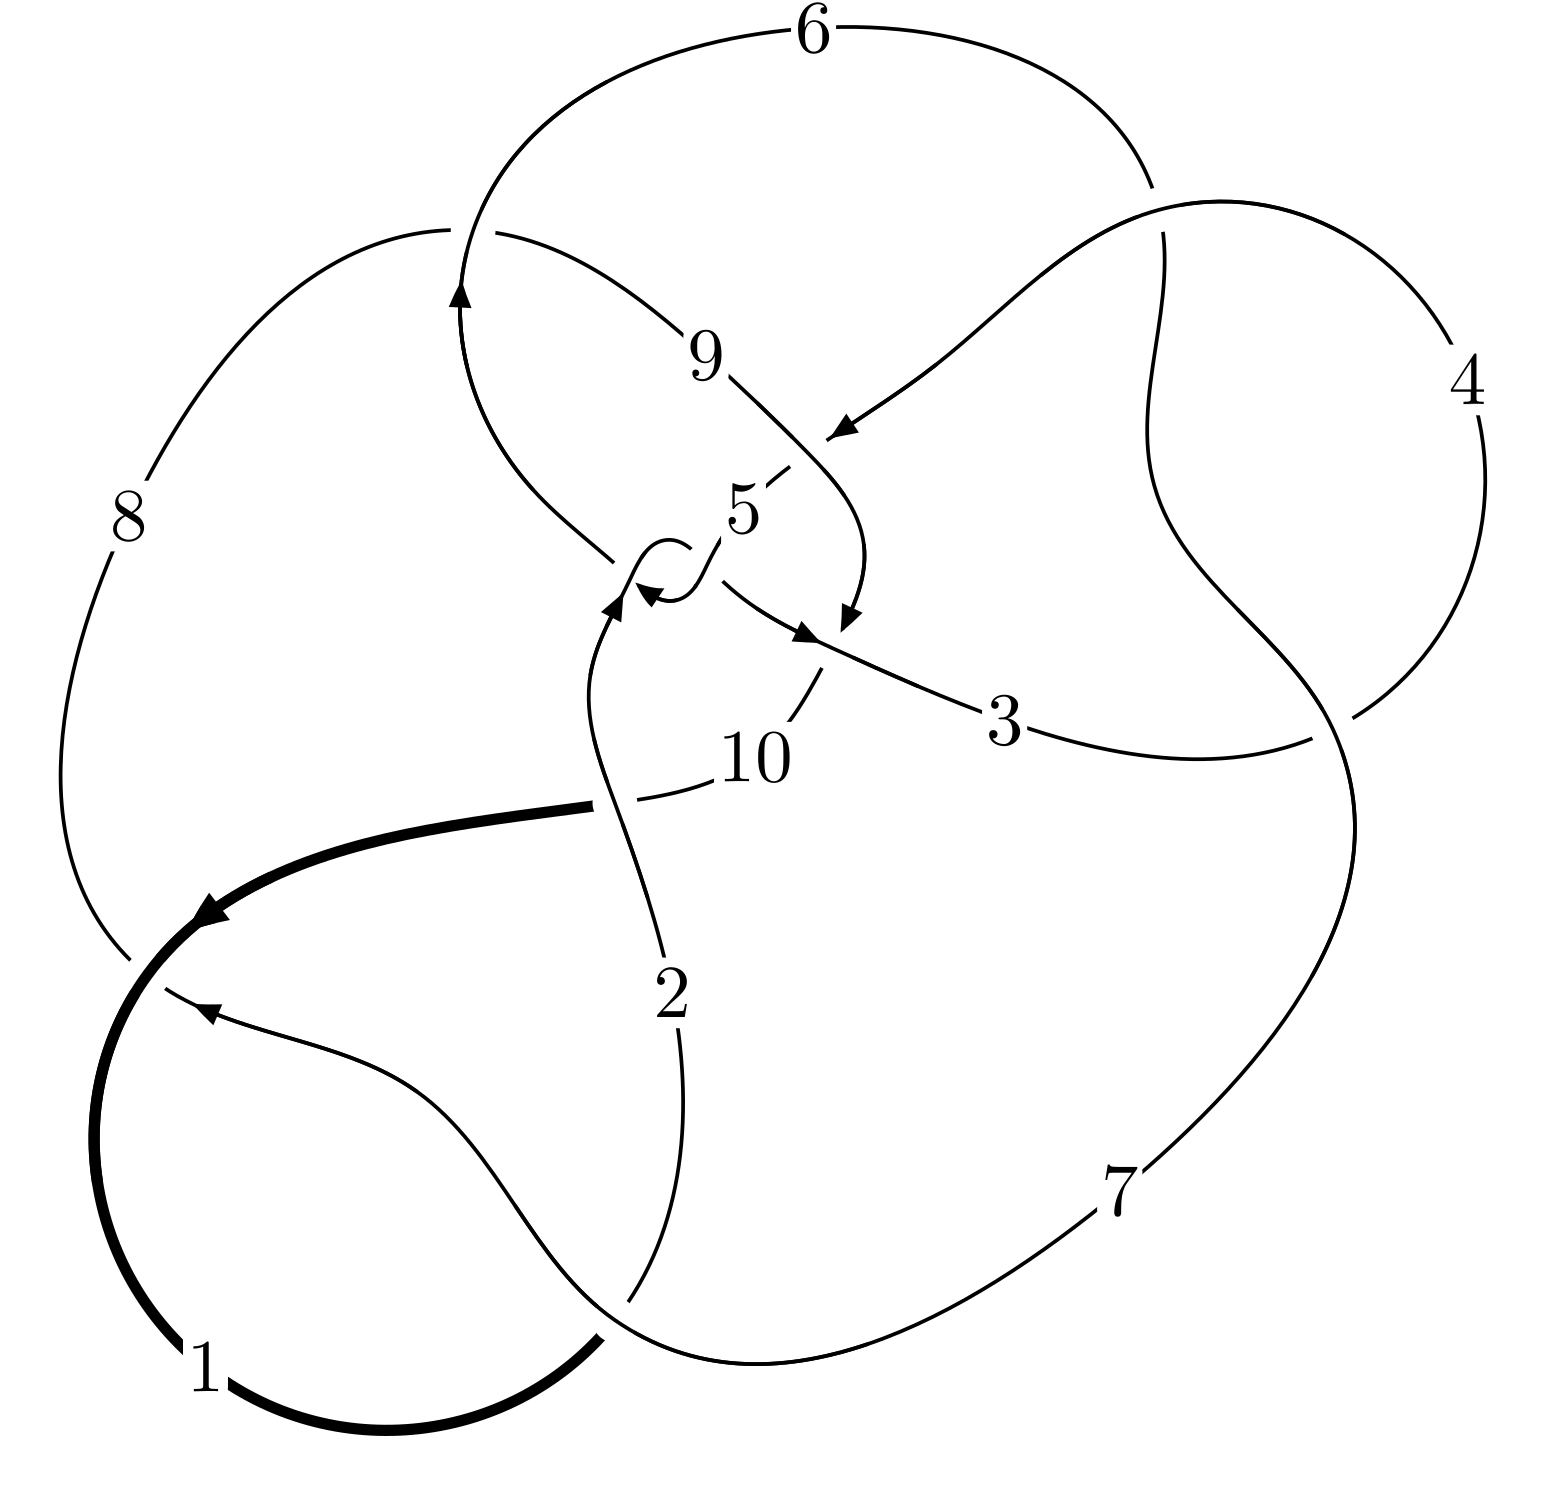
\includegraphics[width=112pt]{../../../GIT/diagram.site/Diagrams/png/230_10_146.png}\\
\ \ \ A knot diagram\footnotemark}&
\allowdisplaybreaks
\textbf{Linearized knot diagam} \\
\cline{2-2}
 &
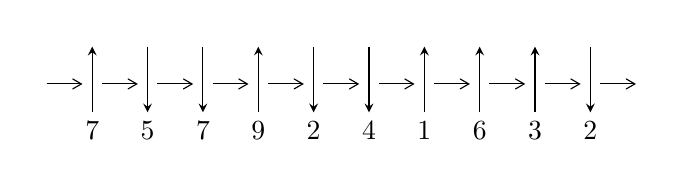
\begin{tikzpicture}[x=20pt, y=17pt]
	% nodes
	\node (C0) at (0, 0) {};
	\node (C1) at (1, 0) {};
	\node (C1U) at (1, +1) {};
	\node (C1D) at (1, -1) {7};

	\node (C2) at (2, 0) {};
	\node (C2U) at (2, +1) {};
	\node (C2D) at (2, -1) {5};

	\node (C3) at (3, 0) {};
	\node (C3U) at (3, +1) {};
	\node (C3D) at (3, -1) {7};

	\node (C4) at (4, 0) {};
	\node (C4U) at (4, +1) {};
	\node (C4D) at (4, -1) {9};

	\node (C5) at (5, 0) {};
	\node (C5U) at (5, +1) {};
	\node (C5D) at (5, -1) {2};

	\node (C6) at (6, 0) {};
	\node (C6U) at (6, +1) {};
	\node (C6D) at (6, -1) {4};

	\node (C7) at (7, 0) {};
	\node (C7U) at (7, +1) {};
	\node (C7D) at (7, -1) {1};

	\node (C8) at (8, 0) {};
	\node (C8U) at (8, +1) {};
	\node (C8D) at (8, -1) {6};

	\node (C9) at (9, 0) {};
	\node (C9U) at (9, +1) {};
	\node (C9D) at (9, -1) {3};

	\node (C10) at (10, 0) {};
	\node (C10U) at (10, +1) {};
	\node (C10D) at (10, -1) {2};
	\node (C11) at (11, 0) {};

	% arrows
	\draw[->,>={angle 60}]
	(C0) edge (C1) (C1) edge (C2) (C2) edge (C3) (C3) edge (C4) (C4) edge (C5) (C5) edge (C6) (C6) edge (C7) (C7) edge (C8) (C8) edge (C9) (C9) edge (C10) (C10) edge (C11) ;	\draw[->,>=stealth]
	(C1D) edge (C1U) (C2U) edge (C2D) (C3U) edge (C3D) (C4D) edge (C4U) (C5U) edge (C5D) (C6U) edge (C6D) (C7D) edge (C7U) (C8D) edge (C8U) (C9D) edge (C9U) (C10U) edge (C10D) ;
	\end{tikzpicture} \\
\hhline{~~} \\& 
\textbf{Solving Sequence} \\ \cline{2-2} 
 &
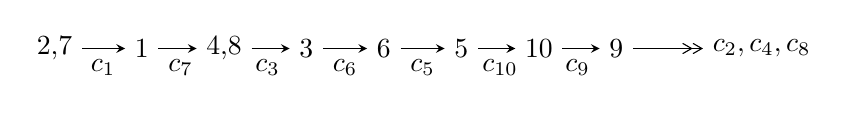
\begin{tikzpicture}[x=28pt, y=7pt]
	% node
	\node (A0) at (-1/8, 0) {2,7};
	\node (A1) at (1, 0) {1};
	\node (A2) at (33/16, 0) {4,8};
	\node (A3) at (25/8, 0) {3};
	\node (A4) at (33/8, 0) {6};
	\node (A5) at (41/8, 0) {5};
	\node (A6) at (49/8, 0) {10};
	\node (A7) at (57/8, 0) {9};
	\node (C1) at (1/2, -1) {$c_{1}$};
	\node (C2) at (3/2, -1) {$c_{7}$};
	\node (C3) at (21/8, -1) {$c_{3}$};
	\node (C4) at (29/8, -1) {$c_{6}$};
	\node (C5) at (37/8, -1) {$c_{5}$};
	\node (C6) at (45/8, -1) {$c_{10}$};
	\node (C7) at (53/8, -1) {$c_{9}$};
	\node (A8) at (9, 0) {$c_{2},c_{4},c_{8}$};

	% edge
	\draw[->,>=stealth]	
	(A0) edge (A1) (A1) edge (A2) (A2) edge (A3) (A3) edge (A4) (A4) edge (A5) (A5) edge (A6) (A6) edge (A7) ;
	\draw[->>,>={angle 60}]	
	(A7) edge (A8);
\end{tikzpicture} \\ 

\end{tabular} \\

\footnotetext{
The image of knot diagram is generated by the software ``\textbf{Draw programme}" developed by Andrew Bartholomew(\url{http://www.layer8.co.uk/maths/draw/index.htm\#Running-draw}), where we modified some parts for our purpose(\url{https://github.com/CATsTAILs/LinksPainter}).
}\phantom \\ \newline 
\centering \textbf{Ideals for irreducible components\footnotemark of $X_{\text{par}}$} 
 
\begin{align*}
I^u_{1}&=\langle 
-469 u^9+1285 u^8+\cdots+1534 b+422,\;-469 u^9+1285 u^8+\cdots+3068 a-1879,\\
\phantom{I^u_{1}}&\phantom{= \langle  }u^{10}-3 u^9+9 u^8-16 u^7+24 u^6-25 u^5+21 u^4-4 u^3-3 u^2+3 u+4\rangle \\
I^u_{2}&=\langle 
b+1,\;3 u^4-2 u^3+a^2+11 u^2- a-5 u+7,\;u^5- u^4+4 u^3-3 u^2+3 u-1\rangle \\
I^u_{3}&=\langle 
- a u+b+a+1,\;a^2- u,\;u^2- u+1\rangle \\
\\
\end{align*}
\raggedright * 3 irreducible components of $\dim_{\mathbb{C}}=0$, with total 24 representations.\\
\footnotetext{All coefficients of polynomials are rational numbers. But the coefficients are sometimes approximated in decimal forms when there is not enough margin.}
\newpage
\renewcommand{\arraystretch}{1}
\centering \section*{I. $I^u_{1}= \langle -469 u^9+1285 u^8+\cdots+1534 b+422,\;-469 u^9+1285 u^8+\cdots+3068 a-1879,\;u^{10}-3 u^9+\cdots+3 u+4 \rangle$}
\flushleft \textbf{(i) Arc colorings}\\
\begin{tabular}{m{7pt} m{180pt} m{7pt} m{180pt} }
\flushright $a_{2}=$&$\begin{pmatrix}1\\0\end{pmatrix}$ \\
\flushright $a_{7}=$&$\begin{pmatrix}0\\u\end{pmatrix}$ \\
\flushright $a_{1}=$&$\begin{pmatrix}1\\u^2\end{pmatrix}$ \\
\flushright $a_{4}=$&$\begin{pmatrix}0.152868 u^{9}-0.418840 u^{8}+\cdots+0.480769 u+0.612451\\0.305737 u^{9}-0.837679 u^{8}+\cdots-1.03846 u-0.275098\end{pmatrix}$ \\
\flushright $a_{8}=$&$\begin{pmatrix}u\\u^3+u\end{pmatrix}$ \\
\flushright $a_{3}=$&$\begin{pmatrix}0.152868 u^{9}-0.418840 u^{8}+\cdots+0.480769 u+0.612451\\0.140808 u^{9}-0.379400 u^{8}+\cdots-0.307692 u-0.116037\end{pmatrix}$ \\
\flushright $a_{6}=$&$\begin{pmatrix}0.0290091 u^{9}+0.0537810 u^{8}+\cdots-0.711538 u-0.220665\\0.0397653 u^{9}+0.0456323 u^{8}+\cdots+0.153846 u-0.611473\end{pmatrix}$ \\
\flushright $a_{5}=$&$\begin{pmatrix}0.0687744 u^{9}+0.0994133 u^{8}+\cdots-0.557692 u-0.832138\\0.0397653 u^{9}+0.0456323 u^{8}+\cdots+0.153846 u-0.611473\end{pmatrix}$ \\
\flushright $a_{10}=$&$\begin{pmatrix}u^2+1\\u^2\end{pmatrix}$ \\
\flushright $a_{9}=$&$\begin{pmatrix}-0.0602999 u^{9}+0.197197 u^{8}+\cdots+1.05769 u+0.857562\\0.0162973 u^{9}+0.108866 u^{8}+\cdots+1.03846 u+0.241199\end{pmatrix}$\\&\end{tabular}
\flushleft \textbf{(ii) Obstruction class $= -1$}\\~\\
\flushleft \textbf{(iii) Cusp Shapes $= \frac{171}{767} u^9-\frac{269}{767} u^8+\frac{1052}{767} u^7-\frac{1818}{767} u^6+\frac{2398}{767} u^5-\frac{4011}{767} u^4+\frac{2685}{767} u^3-\frac{3379}{767} u^2+\frac{37}{13} u-\frac{2378}{767}$}\\~\\
\newpage\renewcommand{\arraystretch}{1}
\flushleft \textbf{(iv) u-Polynomials at the component}\newline \\
\begin{tabular}{m{50pt}|m{274pt}}
Crossings & \hspace{64pt}u-Polynomials at each crossing \\
\hline $$\begin{aligned}c_{1},c_{7}\end{aligned}$$&$\begin{aligned}
&u^{10}-3 u^9+9 u^8-16 u^7+24 u^6-25 u^5+21 u^4-4 u^3-3 u^2+3 u+4
\end{aligned}$\\
\hline $$\begin{aligned}c_{2},c_{3},c_{5}\\c_{6}\end{aligned}$$&$\begin{aligned}
&u^{10}+u^8+u^7+5 u^6+2 u^4+3 u^3+2 u^2+1
\end{aligned}$\\
\hline $$\begin{aligned}c_{4}\end{aligned}$$&$\begin{aligned}
&u^{10}-3 u^9+3 u^8+2 u^7-6 u^6+3 u^5+3 u^4-4 u^3+3 u^2-3 u+2
\end{aligned}$\\
\hline $$\begin{aligned}c_{8},c_{9}\end{aligned}$$&$\begin{aligned}
&u^{10}+2 u^9+9 u^8+7 u^7+30 u^6+6 u^5+41 u^4+22 u^2+4
\end{aligned}$\\
\hline $$\begin{aligned}c_{10}\end{aligned}$$&$\begin{aligned}
&u^{10}+9 u^9+\cdots-33 u+16
\end{aligned}$\\
\hline
\end{tabular}\\~\\
\newpage\renewcommand{\arraystretch}{1}
\flushleft \textbf{(v) Riley Polynomials at the component}\newline \\
\begin{tabular}{m{50pt}|m{274pt}}
Crossings & \hspace{64pt}Riley Polynomials at each crossing \\
\hline $$\begin{aligned}c_{1},c_{7}\end{aligned}$$&$\begin{aligned}
&y^{10}+9 y^9+\cdots-33 y+16
\end{aligned}$\\
\hline $$\begin{aligned}c_{2},c_{3},c_{5}\\c_{6}\end{aligned}$$&$\begin{aligned}
&y^{10}+2 y^9+11 y^8+13 y^7+33 y^6+20 y^5+26 y^4+9 y^3+8 y^2+4 y+1
\end{aligned}$\\
\hline $$\begin{aligned}c_{4}\end{aligned}$$&$\begin{aligned}
&y^{10}-3 y^9+9 y^8-16 y^7+24 y^6-25 y^5+21 y^4-4 y^3-3 y^2+3 y+4
\end{aligned}$\\
\hline $$\begin{aligned}c_{8},c_{9}\end{aligned}$$&$\begin{aligned}
&y^{10}+14 y^9+\cdots+176 y+16
\end{aligned}$\\
\hline $$\begin{aligned}c_{10}\end{aligned}$$&$\begin{aligned}
&y^{10}-15 y^9+\cdots+5343 y+256
\end{aligned}$\\
\hline
\end{tabular}\\~\\
\newpage\flushleft \textbf{(vi) Complex Volumes and Cusp Shapes}
$$\begin{array}{c|c|c}  
\text{Solutions to }I^u_{1}& \I (\text{vol} + \sqrt{-1}CS) & \text{Cusp shape}\\
 \hline 
\begin{aligned}
u &= \phantom{-}0.741866 + 0.796341 I \\
a &= \phantom{-}0.500393 + 0.239842 I \\
b &= -0.625089 + 0.778917 I\end{aligned}
 & \phantom{-}1.60483 + 1.51336 I & \phantom{-}1.256588 - 0.171947 I \\ \hline\begin{aligned}
u &= \phantom{-}0.741866 - 0.796341 I \\
a &= \phantom{-}0.500393 - 0.239842 I \\
b &= -0.625089 - 0.778917 I\end{aligned}
 & \phantom{-}1.60483 - 1.51336 I & \phantom{-}1.256588 + 0.171947 I \\ \hline\begin{aligned}
u &= \phantom{-}1.077560 + 0.740596 I \\
a &= \phantom{-}0.030843 - 0.749210 I \\
b &= \phantom{-}0.94514 - 1.33248 I\end{aligned}
 & \phantom{-}1.74604 + 4.90489 I & \phantom{-}2.53483 - 7.39457 I \\ \hline\begin{aligned}
u &= \phantom{-}1.077560 - 0.740596 I \\
a &= \phantom{-}0.030843 + 0.749210 I \\
b &= \phantom{-}0.94514 + 1.33248 I\end{aligned}
 & \phantom{-}1.74604 - 4.90489 I & \phantom{-}2.53483 + 7.39457 I \\ \hline\begin{aligned}
u &= -0.429682 + 0.277960 I \\
a &= \phantom{-}0.69620 + 1.42291 I \\
b &= \phantom{-}0.722559 + 0.567039 I\end{aligned}
 & -1.23090 - 1.07704 I & -4.33290 + 2.58024 I \\ \hline\begin{aligned}
u &= -0.429682 - 0.277960 I \\
a &= \phantom{-}0.69620 - 1.42291 I \\
b &= \phantom{-}0.722559 - 0.567039 I\end{aligned}
 & -1.23090 + 1.07704 I & -4.33290 - 2.58024 I \\ \hline\begin{aligned}
u &= -0.25937 + 1.52583 I \\
a &= -0.571923 + 0.727637 I \\
b &= \phantom{-}1.66770 + 0.84950 I\end{aligned}
 & -7.19127 - 3.97850 I & -1.38540 + 2.06163 I \\ \hline\begin{aligned}
u &= -0.25937 - 1.52583 I \\
a &= -0.571923 - 0.727637 I \\
b &= \phantom{-}1.66770 - 0.84950 I\end{aligned}
 & -7.19127 + 3.97850 I & -1.38540 - 2.06163 I \\ \hline\begin{aligned}
u &= \phantom{-}0.36963 + 1.73551 I \\
a &= -0.530514 - 0.624791 I \\
b &= \phantom{-}1.78968 - 0.93001 I\end{aligned}
 & -6.44324 + 10.56100 I & -0.07312 - 6.56398 I \\ \hline\begin{aligned}
u &= \phantom{-}0.36963 - 1.73551 I \\
a &= -0.530514 + 0.624791 I \\
b &= \phantom{-}1.78968 + 0.93001 I\end{aligned}
 & -6.44324 - 10.56100 I & -0.07312 + 6.56398 I\\
 \hline 
 \end{array}$$\newpage\newpage\renewcommand{\arraystretch}{1}
\centering \section*{II. $I^u_{2}= \langle b+1,\;3 u^4-2 u^3+a^2+11 u^2- a-5 u+7,\;u^5- u^4+4 u^3-3 u^2+3 u-1 \rangle$}
\flushleft \textbf{(i) Arc colorings}\\
\begin{tabular}{m{7pt} m{180pt} m{7pt} m{180pt} }
\flushright $a_{2}=$&$\begin{pmatrix}1\\0\end{pmatrix}$ \\
\flushright $a_{7}=$&$\begin{pmatrix}0\\u\end{pmatrix}$ \\
\flushright $a_{1}=$&$\begin{pmatrix}1\\u^2\end{pmatrix}$ \\
\flushright $a_{4}=$&$\begin{pmatrix}a\\-1\end{pmatrix}$ \\
\flushright $a_{8}=$&$\begin{pmatrix}u\\u^3+u\end{pmatrix}$ \\
\flushright $a_{3}=$&$\begin{pmatrix}a\\- u^2 a-1\end{pmatrix}$ \\
\flushright $a_{6}=$&$\begin{pmatrix}- u^4+u^3+a u-4 u^2+2 u-3\\- a u+u\end{pmatrix}$ \\
\flushright $a_{5}=$&$\begin{pmatrix}- u^4+u^3-4 u^2+3 u-3\\- a u+u\end{pmatrix}$ \\
\flushright $a_{10}=$&$\begin{pmatrix}u^2+1\\u^2\end{pmatrix}$ \\
\flushright $a_{9}=$&$\begin{pmatrix}- u^4 a+u^4-3 u^2 a+4 u^2- a+3\\u^4 a- u^3 a+3 u^2 a+u^3-2 a u+a+2 u\end{pmatrix}$\\&\end{tabular}
\flushleft \textbf{(ii) Obstruction class $= -1$}\\~\\
\flushleft \textbf{(iii) Cusp Shapes $= 4 u^4-4 u^3+16 u^2-12 u+10$}\\~\\
\newpage\renewcommand{\arraystretch}{1}
\flushleft \textbf{(iv) u-Polynomials at the component}\newline \\
\begin{tabular}{m{50pt}|m{274pt}}
Crossings & \hspace{64pt}u-Polynomials at each crossing \\
\hline $$\begin{aligned}c_{1},c_{7}\end{aligned}$$&$\begin{aligned}
&(u^5- u^4+4 u^3-3 u^2+3 u-1)^2
\end{aligned}$\\
\hline $$\begin{aligned}c_{2},c_{3},c_{5}\\c_{6}\end{aligned}$$&$\begin{aligned}
&u^{10}- u^9+2 u^8-2 u^7+4 u^6-4 u^5+9 u^4-7 u^3+8 u^2-4 u+1
\end{aligned}$\\
\hline $$\begin{aligned}c_{4}\end{aligned}$$&$\begin{aligned}
&(u^5+u^4- u^2+u+1)^2
\end{aligned}$\\
\hline $$\begin{aligned}c_{8},c_{9}\end{aligned}$$&$\begin{aligned}
&u^{10}+u^9+2 u^8-2 u^7+6 u^6+10 u^5+11 u^4+27 u^3+6 u^2+10 u+29
\end{aligned}$\\
\hline $$\begin{aligned}c_{10}\end{aligned}$$&$\begin{aligned}
&(u^5+7 u^4+16 u^3+13 u^2+3 u-1)^2
\end{aligned}$\\
\hline
\end{tabular}\\~\\
\newpage\renewcommand{\arraystretch}{1}
\flushleft \textbf{(v) Riley Polynomials at the component}\newline \\
\begin{tabular}{m{50pt}|m{274pt}}
Crossings & \hspace{64pt}Riley Polynomials at each crossing \\
\hline $$\begin{aligned}c_{1},c_{7}\end{aligned}$$&$\begin{aligned}
&(y^5+7 y^4+16 y^3+13 y^2+3 y-1)^2
\end{aligned}$\\
\hline $$\begin{aligned}c_{2},c_{3},c_{5}\\c_{6}\end{aligned}$$&$\begin{aligned}
&y^{10}+3 y^9+8 y^8+22 y^7+38 y^6+54 y^5+77 y^4+71 y^3+26 y^2+1
\end{aligned}$\\
\hline $$\begin{aligned}c_{4}\end{aligned}$$&$\begin{aligned}
&(y^5- y^4+4 y^3-3 y^2+3 y-1)^2
\end{aligned}$\\
\hline $$\begin{aligned}c_{8},c_{9}\end{aligned}$$&$\begin{aligned}
&y^{10}+3 y^9+\cdots+248 y+841
\end{aligned}$\\
\hline $$\begin{aligned}c_{10}\end{aligned}$$&$\begin{aligned}
&(y^5-17 y^4+80 y^3-59 y^2+35 y-1)^2
\end{aligned}$\\
\hline
\end{tabular}\\~\\
\newpage\flushleft \textbf{(vi) Complex Volumes and Cusp Shapes}
$$\begin{array}{c|c|c}  
\text{Solutions to }I^u_{2}& \I (\text{vol} + \sqrt{-1}CS) & \text{Cusp shape}\\
 \hline 
\begin{aligned}
u &= \phantom{-}0.233677 + 0.885557 I \\
a &= \phantom{-}1.186080 + 0.428672 I \\
b &= -1.00000\phantom{ +0.000000I}\end{aligned}
 & \phantom{-}1.47006 + 2.21397 I & -0.88568 - 4.22289 I \\ \hline\begin{aligned}
u &= \phantom{-}0.233677 + 0.885557 I \\
a &= -0.186079 - 0.428672 I \\
b &= -1.00000\phantom{ +0.000000I}\end{aligned}
 & \phantom{-}1.47006 + 2.21397 I & -0.88568 - 4.22289 I \\ \hline\begin{aligned}
u &= \phantom{-}0.233677 - 0.885557 I \\
a &= \phantom{-}1.186080 - 0.428672 I \\
b &= -1.00000\phantom{ +0.000000I}\end{aligned}
 & \phantom{-}1.47006 - 2.21397 I & -0.88568 + 4.22289 I \\ \hline\begin{aligned}
u &= \phantom{-}0.233677 - 0.885557 I \\
a &= -0.186079 + 0.428672 I \\
b &= -1.00000\phantom{ +0.000000I}\end{aligned}
 & \phantom{-}1.47006 - 2.21397 I & -0.88568 + 4.22289 I \\ \hline\begin{aligned}
u &= \phantom{-}0.416284\phantom{ +0.000000I} \\
a &= \phantom{-}0.50000 + 2.55355 I \\
b &= -1.00000\phantom{ +0.000000I}\end{aligned}
 & \phantom{-}4.17205\phantom{ +0.000000I} & \phantom{-}7.60880\phantom{ +0.000000I} \\ \hline\begin{aligned}
u &= \phantom{-}0.416284\phantom{ +0.000000I} \\
a &= \phantom{-}0.50000 - 2.55355 I \\
b &= -1.00000\phantom{ +0.000000I}\end{aligned}
 & \phantom{-}4.17205\phantom{ +0.000000I} & \phantom{-}7.60880\phantom{ +0.000000I} \\ \hline\begin{aligned}
u &= \phantom{-}0.05818 + 1.69128 I \\
a &= \phantom{-}0.518923 + 0.634033 I \\
b &= -1.00000\phantom{ +0.000000I}\end{aligned}
 & -7.66842 + 3.33174 I & -1.91874 - 2.36228 I \\ \hline\begin{aligned}
u &= \phantom{-}0.05818 + 1.69128 I \\
a &= \phantom{-}0.481077 - 0.634033 I \\
b &= -1.00000\phantom{ +0.000000I}\end{aligned}
 & -7.66842 + 3.33174 I & -1.91874 - 2.36228 I \\ \hline\begin{aligned}
u &= \phantom{-}0.05818 - 1.69128 I \\
a &= \phantom{-}0.518923 - 0.634033 I \\
b &= -1.00000\phantom{ +0.000000I}\end{aligned}
 & -7.66842 - 3.33174 I & -1.91874 + 2.36228 I \\ \hline\begin{aligned}
u &= \phantom{-}0.05818 - 1.69128 I \\
a &= \phantom{-}0.481077 + 0.634033 I \\
b &= -1.00000\phantom{ +0.000000I}\end{aligned}
 & -7.66842 - 3.33174 I & -1.91874 + 2.36228 I\\
 \hline 
 \end{array}$$\newpage\newpage\renewcommand{\arraystretch}{1}
\centering \section*{III. $I^u_{3}= \langle - a u+b+a+1,\;a^2- u,\;u^2- u+1 \rangle$}
\flushleft \textbf{(i) Arc colorings}\\
\begin{tabular}{m{7pt} m{180pt} m{7pt} m{180pt} }
\flushright $a_{2}=$&$\begin{pmatrix}1\\0\end{pmatrix}$ \\
\flushright $a_{7}=$&$\begin{pmatrix}0\\u\end{pmatrix}$ \\
\flushright $a_{1}=$&$\begin{pmatrix}1\\u-1\end{pmatrix}$ \\
\flushright $a_{4}=$&$\begin{pmatrix}a\\a u- a-1\end{pmatrix}$ \\
\flushright $a_{8}=$&$\begin{pmatrix}u\\u-1\end{pmatrix}$ \\
\flushright $a_{3}=$&$\begin{pmatrix}a\\-1\end{pmatrix}$ \\
\flushright $a_{6}=$&$\begin{pmatrix}u-1\\- a u\end{pmatrix}$ \\
\flushright $a_{5}=$&$\begin{pmatrix}- a u+u-1\\- a u\end{pmatrix}$ \\
\flushright $a_{10}=$&$\begin{pmatrix}u\\u-1\end{pmatrix}$ \\
\flushright $a_{9}=$&$\begin{pmatrix}- a u+u+1\\a u- a+2 u-1\end{pmatrix}$\\&\end{tabular}
\flushleft \textbf{(ii) Obstruction class $= 1$}\\~\\
\flushleft \textbf{(iii) Cusp Shapes $= -4 u+8$}\\~\\
\newpage\renewcommand{\arraystretch}{1}
\flushleft \textbf{(iv) u-Polynomials at the component}\newline \\
\begin{tabular}{m{50pt}|m{274pt}}
Crossings & \hspace{64pt}u-Polynomials at each crossing \\
\hline $$\begin{aligned}c_{1},c_{10}\end{aligned}$$&$\begin{aligned}
&(u^2- u+1)^2
\end{aligned}$\\
\hline $$\begin{aligned}c_{2},c_{3},c_{5}\\c_{6}\end{aligned}$$&$\begin{aligned}
&(u^2+1)^2
\end{aligned}$\\
\hline $$\begin{aligned}c_{4}\end{aligned}$$&$\begin{aligned}
&u^4- u^2+1
\end{aligned}$\\
\hline $$\begin{aligned}c_{7}\end{aligned}$$&$\begin{aligned}
&(u^2+u+1)^2
\end{aligned}$\\
\hline $$\begin{aligned}c_{8}\end{aligned}$$&$\begin{aligned}
&u^4-2 u^3+2 u^2-4 u+4
\end{aligned}$\\
\hline $$\begin{aligned}c_{9}\end{aligned}$$&$\begin{aligned}
&u^4+2 u^3+2 u^2+4 u+4
\end{aligned}$\\
\hline
\end{tabular}\\~\\
\newpage\renewcommand{\arraystretch}{1}
\flushleft \textbf{(v) Riley Polynomials at the component}\newline \\
\begin{tabular}{m{50pt}|m{274pt}}
Crossings & \hspace{64pt}Riley Polynomials at each crossing \\
\hline $$\begin{aligned}c_{1},c_{7},c_{10}\end{aligned}$$&$\begin{aligned}
&(y^2+y+1)^2
\end{aligned}$\\
\hline $$\begin{aligned}c_{2},c_{3},c_{5}\\c_{6}\end{aligned}$$&$\begin{aligned}
&(y+1)^4
\end{aligned}$\\
\hline $$\begin{aligned}c_{4}\end{aligned}$$&$\begin{aligned}
&(y^2- y+1)^2
\end{aligned}$\\
\hline $$\begin{aligned}c_{8},c_{9}\end{aligned}$$&$\begin{aligned}
&y^4-4 y^2+16
\end{aligned}$\\
\hline
\end{tabular}\\~\\
\newpage\flushleft \textbf{(vi) Complex Volumes and Cusp Shapes}
$$\begin{array}{c|c|c}  
\text{Solutions to }I^u_{3}& \I (\text{vol} + \sqrt{-1}CS) & \text{Cusp shape}\\
 \hline 
\begin{aligned}
u &= \phantom{-}0.500000 + 0.866025 I \\
a &= \phantom{-}0.866025 + 0.500000 I \\
b &= -1.86603 + 0.50000 I\end{aligned}
 & \phantom{-}3.28987 + 2.02988 I & \phantom{-}6.00000 - 3.46410 I \\ \hline\begin{aligned}
u &= \phantom{-}0.500000 + 0.866025 I \\
a &= -0.866025 - 0.500000 I \\
b &= -0.133975 - 0.500000 I\end{aligned}
 & \phantom{-}3.28987 + 2.02988 I & \phantom{-}6.00000 - 3.46410 I \\ \hline\begin{aligned}
u &= \phantom{-}0.500000 - 0.866025 I \\
a &= \phantom{-}0.866025 - 0.500000 I \\
b &= -1.86603 - 0.50000 I\end{aligned}
 & \phantom{-}3.28987 - 2.02988 I & \phantom{-}6.00000 + 3.46410 I \\ \hline\begin{aligned}
u &= \phantom{-}0.500000 - 0.866025 I \\
a &= -0.866025 + 0.500000 I \\
b &= -0.133975 + 0.500000 I\end{aligned}
 & \phantom{-}3.28987 - 2.02988 I & \phantom{-}6.00000 + 3.46410 I\\
 \hline 
 \end{array}$$\newpage
\newpage\renewcommand{\arraystretch}{1}
\centering \section*{ IV. u-Polynomials}
\begin{tabular}{m{50pt}|m{274pt}}
Crossings & \hspace{64pt}u-Polynomials at each crossing \\
\hline $$\begin{aligned}c_{1}\end{aligned}$$&$\begin{aligned}
&(u^2- u+1)^2(u^5- u^4+4 u^3-3 u^2+3 u-1)^2\\
&\cdot(u^{10}-3 u^9+9 u^8-16 u^7+24 u^6-25 u^5+21 u^4-4 u^3-3 u^2+3 u+4)
\end{aligned}$\\
\hline $$\begin{aligned}c_{2},c_{3},c_{5}\\c_{6}\end{aligned}$$&$\begin{aligned}
&(u^2+1)^2(u^{10}+u^8+u^7+5 u^6+2 u^4+3 u^3+2 u^2+1)\\
&\cdot(u^{10}- u^9+2 u^8-2 u^7+4 u^6-4 u^5+9 u^4-7 u^3+8 u^2-4 u+1)
\end{aligned}$\\
\hline $$\begin{aligned}c_{4}\end{aligned}$$&$\begin{aligned}
&(u^4- u^2+1)(u^5+u^4- u^2+u+1)^2\\
&\cdot(u^{10}-3 u^9+3 u^8+2 u^7-6 u^6+3 u^5+3 u^4-4 u^3+3 u^2-3 u+2)
\end{aligned}$\\
\hline $$\begin{aligned}c_{7}\end{aligned}$$&$\begin{aligned}
&(u^2+u+1)^2(u^5- u^4+4 u^3-3 u^2+3 u-1)^2\\
&\cdot(u^{10}-3 u^9+9 u^8-16 u^7+24 u^6-25 u^5+21 u^4-4 u^3-3 u^2+3 u+4)
\end{aligned}$\\
\hline $$\begin{aligned}c_{8}\end{aligned}$$&$\begin{aligned}
&(u^4-2 u^3+2 u^2-4 u+4)\\
&\cdot(u^{10}+u^9+2 u^8-2 u^7+6 u^6+10 u^5+11 u^4+27 u^3+6 u^2+10 u+29)\\
&\cdot(u^{10}+2 u^9+9 u^8+7 u^7+30 u^6+6 u^5+41 u^4+22 u^2+4)
\end{aligned}$\\
\hline $$\begin{aligned}c_{9}\end{aligned}$$&$\begin{aligned}
&(u^4+2 u^3+2 u^2+4 u+4)\\
&\cdot(u^{10}+u^9+2 u^8-2 u^7+6 u^6+10 u^5+11 u^4+27 u^3+6 u^2+10 u+29)\\
&\cdot(u^{10}+2 u^9+9 u^8+7 u^7+30 u^6+6 u^5+41 u^4+22 u^2+4)
\end{aligned}$\\
\hline $$\begin{aligned}c_{10}\end{aligned}$$&$\begin{aligned}
&(u^2- u+1)^2(u^5+7 u^4+16 u^3+13 u^2+3 u-1)^2\\
&\cdot(u^{10}+9 u^9+\cdots-33 u+16)
\end{aligned}$\\
\hline
\end{tabular}\newpage\renewcommand{\arraystretch}{1}
\centering \section*{ V. Riley Polynomials}
\begin{tabular}{m{50pt}|m{274pt}}
Crossings & \hspace{64pt}Riley Polynomials at each crossing \\
\hline $$\begin{aligned}c_{1},c_{7}\end{aligned}$$&$\begin{aligned}
&(y^2+y+1)^2(y^5+7 y^4+16 y^3+13 y^2+3 y-1)^2\\
&\cdot(y^{10}+9 y^9+\cdots-33 y+16)
\end{aligned}$\\
\hline $$\begin{aligned}c_{2},c_{3},c_{5}\\c_{6}\end{aligned}$$&$\begin{aligned}
&(y+1)^4\\
&\cdot(y^{10}+2 y^9+11 y^8+13 y^7+33 y^6+20 y^5+26 y^4+9 y^3+8 y^2+4 y+1)\\
&\cdot(y^{10}+3 y^9+8 y^8+22 y^7+38 y^6+54 y^5+77 y^4+71 y^3+26 y^2+1)
\end{aligned}$\\
\hline $$\begin{aligned}c_{4}\end{aligned}$$&$\begin{aligned}
&(y^2- y+1)^2(y^5- y^4+4 y^3-3 y^2+3 y-1)^2\\
&\cdot(y^{10}-3 y^9+9 y^8-16 y^7+24 y^6-25 y^5+21 y^4-4 y^3-3 y^2+3 y+4)
\end{aligned}$\\
\hline $$\begin{aligned}c_{8},c_{9}\end{aligned}$$&$\begin{aligned}
&(y^4-4 y^2+16)(y^{10}+3 y^9+\cdots+248 y+841)\\
&\cdot(y^{10}+14 y^9+\cdots+176 y+16)
\end{aligned}$\\
\hline $$\begin{aligned}c_{10}\end{aligned}$$&$\begin{aligned}
&(y^2+y+1)^2(y^5-17 y^4+80 y^3-59 y^2+35 y-1)^2\\
&\cdot(y^{10}-15 y^9+\cdots+5343 y+256)
\end{aligned}$\\
\hline
\end{tabular}
\vskip 2pc
\end{document}